\documentclass[12pt, a4paper, oneside, titlepage]{report}
\special{papersize=9in,11in}

\usepackage[utf8]{inputenc}
\usepackage{titlesec}
\usepackage{coverpage}
\usepackage[paperwidth=9in, paperheight=11in, margin=1in]{geometry}
\usepackage[bookmarks, hidelinks]{hyperref}
%\usepackage{blindtext}
\usepackage[nonumberlist]{glossaries}
\usepackage{listings}
\usepackage{graphicx}


\newcommand{\blindtext}[0]{}
% define glossary items
\makeglossaries
% vi:ft=tex

\newglossaryentry{pbs}{
    name=Portable Batch System,
    symbol=PBS,
    description={A workload manager}
}

\newglossaryentry{hpc}{
    name=High Performance Computing,
    symbol=HPC,
    description={
        High-performance computing is the use of parallel processing
        for running advanced application programs efficiently, reliably and
        quickly.
    }
}

\newglossaryentry{job}{
    name=job,
    description={A program run on a computer.}
}

\newglossaryentry{spark}{
    name=Spark,
    description={A Big Data analytics thing}
}

\newglossaryentry{executor}{
    name={Spark Executor},
    description=executor,
    plural={Spark Executors},
}

\newglossaryentry{walltime}{
    name=walltime,
    description={what is walltime},
}

\newglossaryentry{yarn}{
    name=Apache Hadoop Yarn,
    description=todo.
}

\newglossaryentry{mesos}{
    name=Apache Mesos,
    description=todo.
}

\newglossaryentry{kubernetes}{
    name=Kubernetes,
    description=todo.
}

\newglossaryentry{driver}{
    name=Spark Driver,
    description=todo,
}



\title{Addition of \gls{pbs} as a cluster manager in Apache \gls{spark}}
\author{Utkarsh Maheshwari}

\titleformat{\chapter}[display]
  {\normalfont\bfseries}{}{0pt}{\Huge}

\begin{document}

\makecover
\maketitlepage
\makeabstract

\chapter{Acknowledgements}

THIS SECTION IS WORK IN PROGRESS\\

Thanks given to:\\
• Head of the organisation,\\
• Co-ordinator of the PS programme at the organisation,\\
• Professional Expert / Incharge of the project,\\
• PS Faculty,\\
• Other persons (from the organisation and /or outside the organisation, etc.)\\


\tableofcontents
\addtocounter{chapter}{1}
\addcontentsline{toc}{chapter}{\protect\numberline{\thechapter}Contents}

\chapter{Introduction}
% vi:ft=tex

\section{About Apache Spark?}

\paragraph{} \Gls{spark} is the leading frontrunner in Big Data Analytics and
Machine Learning. A \gls{spark} application can run for days crunching on data
and churning out results. This is why most \gls{spark} applications utilize a
cluster of nodes to execute tasks to decrease the time. A \gls{spark} cluster
can be set up using its own cluster manager known as \gls{spark} Standalone
Cluster Manager or one of third party cluster managers like \gls{yarn},
\gls{mesos} or \gls{kubernetes}.


\section{About \glssymbol{pbs}}

\paragraph{} \glssymbol{pbs} is a workload management system which optimizes
\gls{job} scheduling in \gls{hpc} environments --- clusters, clouds and super
computers. A \glssymbol{pbs} job can be anything from a batch script to a C/C++
application. It is an open sourced application with commercial support also
available which can be run on Linux or Windows platforms.


\section{Need for adding \glssymbol{pbs} as a cluster manager in \gls{spark}}

\paragraph{} There are many organizations which require running \gls{hpc} jobs
as well as Big Data jobs on a cluster. But none of the cluster managers which
integrate with \gls{spark} are capable of running an \gls{hpc} job, thus
creating a need to add \gls{pbs} as a pluggable scheduler in \gls{spark}. This
project aims to do just that.


\chapter{Project details}
% vi:ft=tex

\section{Problem statement}

\paragraph{}
\glssymbol{pbs} is a workload management system which optimizes \gls{job}
scheduling in \gls{hpc} environments --- clusters, clouds and super computers.
\gls{spark} is a data analytics engine for large-scale data processing and has a
standalone cluster manager which handles the spark jobs sent to a cluster of
nodes. But for both of these, their own daemons should be running on the nodes
and should have information about the node like number of CPU cores, memory
available for use etc. Since they are two completely different programs, they
have no way of knowing which node is in use by the other program at a given time
and thus create problems when scheduling.

\paragraph{}
The current workaround for the said problem is to segregate the nodes cluster
into two partitions --- \glssymbol{hpc} cluster and \gls{spark} cluster. But
this creates another problem. At any given time if the demand for running
\glssymbol{hpc} jobs is high and the demand for \gls{spark} jobs is low, the
\gls{spark} cluster will remain idle while \glssymbol{hpc} jobs may end up in
queued state. This is a gross underutilization of the cluster for which the
organization is paying but is unable to efficiently use.


\section{Potential solutions}

The potential solutions to this problem can be:
\begin{enumerate}
    \item Running a \gls{executor} on the \glssymbol{pbs} cluster
        endlessly. This can be done without modifying any code anywhere but it
        increases the need for human interaction. \glssymbol{pbs} jobs also
        have a \gls{walltime} for all jobs. Running a \gls{executor}
        endlessly also violates that condition.
    \item Starting \glspl{executor} as \glssymbol{pbs} jobs on demand.
        This option requires knowing when a \gls{spark} job is submitted and how
        must resources are required for it.
\end{enumerate}


\section{Solution description}

\paragraph{}
The solution which seems most feasible is to start \glspl{executor} on
demand as \glssymbol{hpc} jobs. To do this, we must know how many executors or
memory or CPU cores does the spark application require. This information can
only be acquired if we hack into the \gls{spark} codebase.

\paragraph{}
Please see \hyperref[sec:appendix-spark]{Appendix for \gls{spark}} for more
information on \gls{spark}'s architecture.


\section{Implementation}

\begin{figure}[h]
    \centering
    \fbox{
        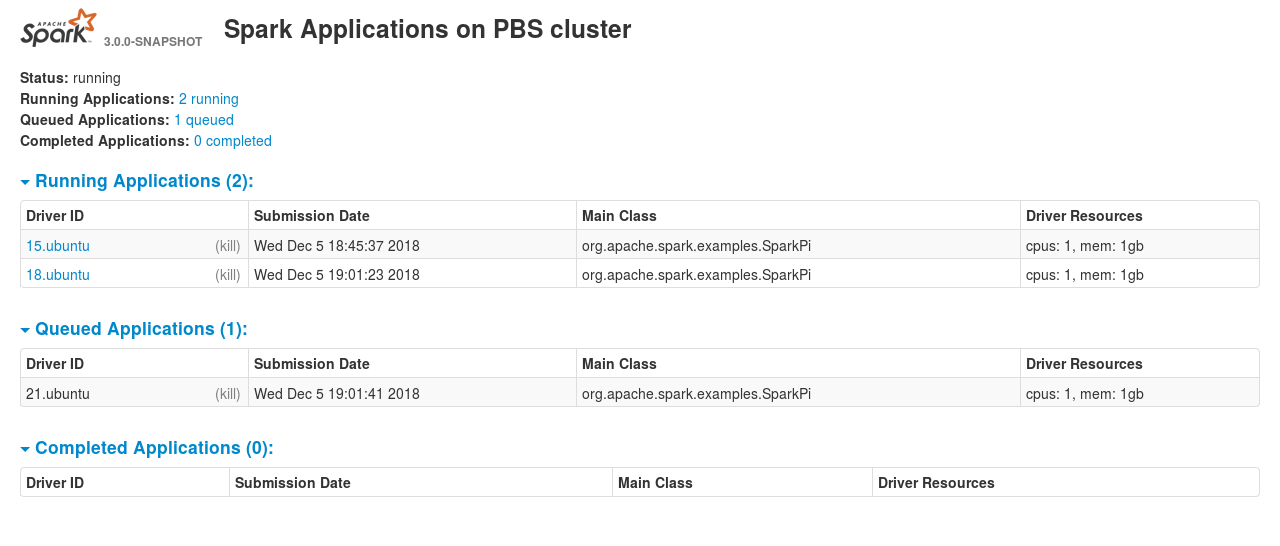
\includegraphics[width=0.75 \textwidth, natwidth=1280, natheight=900]
            {assets/images/Cluster.png}
        }
    \caption{Spark Cluster UI page displaying jobs on PBS Cluster}
\end{figure}

\subsection{Overriding Spark's cluster manager}
\paragraph{}
There is already support in \gls{spark} codebase for \gls{yarn}, \gls{mesos} and
\gls{kubernetes}. This is done by overriding the \texttt{ExternalClusterManager}
in Spark. This class is responsible to create an instance of
\texttt{SchedulerBackend} which we also override. The \texttt{SchedulerBackend}
is responsible to start the \glspl{executor} and we change that so that it
now submits the \glspl{executor} as jobs to \glssymbol{pbs} instead.

\begin{figure}[h]
    \centering
    \fbox{
        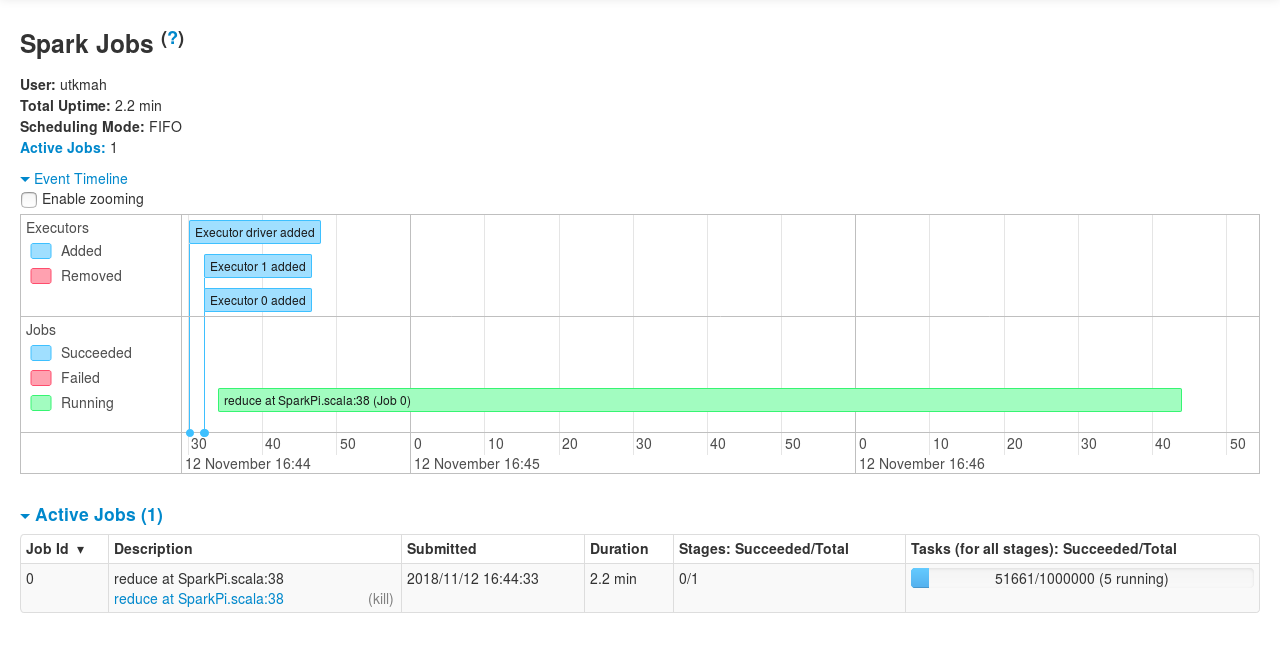
\includegraphics[width=0.75 \textwidth, natwidth=1280, natheight=849]
            {assets/images/Jobs.png}
        }
    \caption{Spark Job page for each Spark Driver}
\end{figure}

\paragraph{}
The above setup works well for a job where the \gls{driver} is run locally. But
to allow the \gls{driver} to run remotely on a cluster, we must also be able to
submit the \gls{driver} as a \glssymbol{pbs} job. To do this, we also override
\texttt{SparkApplication} which is instantiated whenever a \gls{spark} job is
submitted. This is responsible to start the \gls{driver} which we now just start
as a \glssymbol{pbs} job.

\begin{figure}[h]
    \centering
    \fbox{
        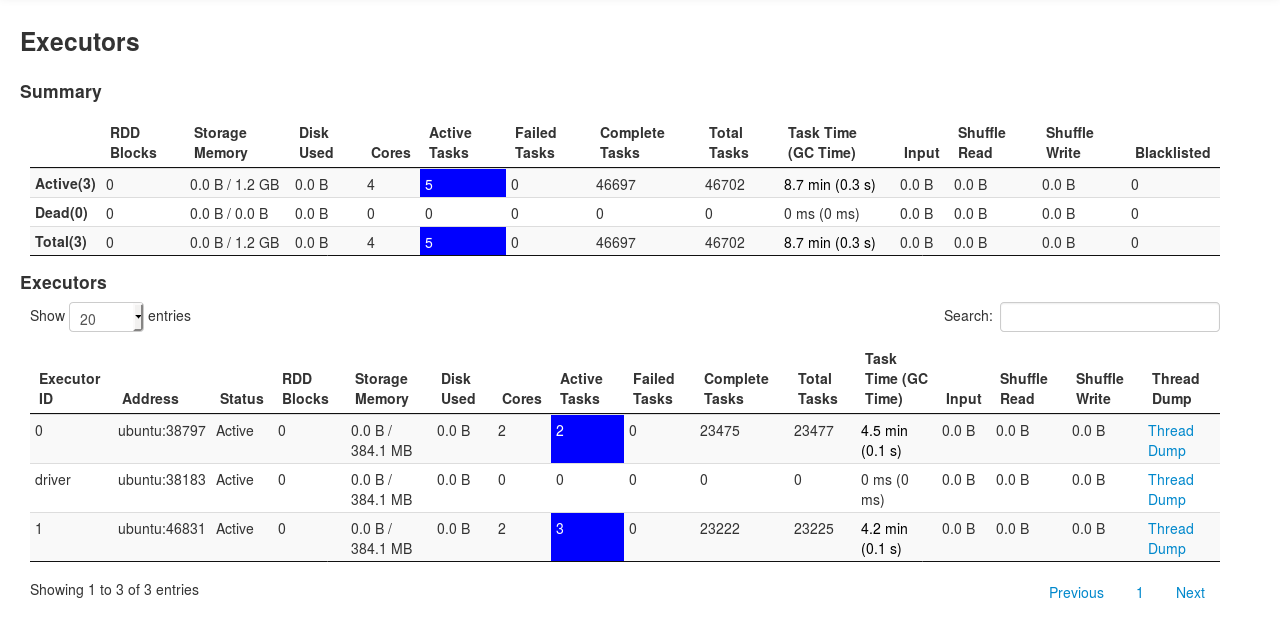
\includegraphics[width=0.75 \textwidth, natwidth=1280, natheight=849]
            {assets/images/Executors.png}
        }
    \caption{Job page listing executors which are running on PBS cluster nodes}
\end{figure}


\section{Result}

\subsection{Installation}
\paragraph{}
The \gls{spark} application has to be patched to allow setting \glssymbol{pbs}
as a scheduler. Apart from this, the \gls{spark} application must be compiled
with the overridden classes. This whole compiled version of \gls{spark} must be
installed on each execution node of the cluster as well as the client node.
In addtion, to submit an application to \gls{spark} on \glssymbol{pbs} cluster,
there must also be a \glssymbol{pbs} client distribution installed on the client
machine.

\subsection{Usage}
\paragraph{}
The \gls{spark} application can be submitted just like it used to be submitted
before the \glssymbol{pbs} integration with the commands following the similar
pattern:

\begin{samepage}
    \begin{itemize}
        \item Submit \gls{spark} application on \glssymbol{pbs} cluster:\\
            \texttt{bin/spark-shell --master pbs}

        \item Submit application with \gls{driver} running locally:\\
            \texttt{bin/spark-submit --master pbs --deploy-mode client}

        \item Submit application with \gls{driver} running on the cluster:\\
            \texttt{bin/spark-submit --master pbs --deploy-mode cluster}
    \end{itemize}
\end{samepage}


\begin{figure}[h]
    \centering
    \fbox{
        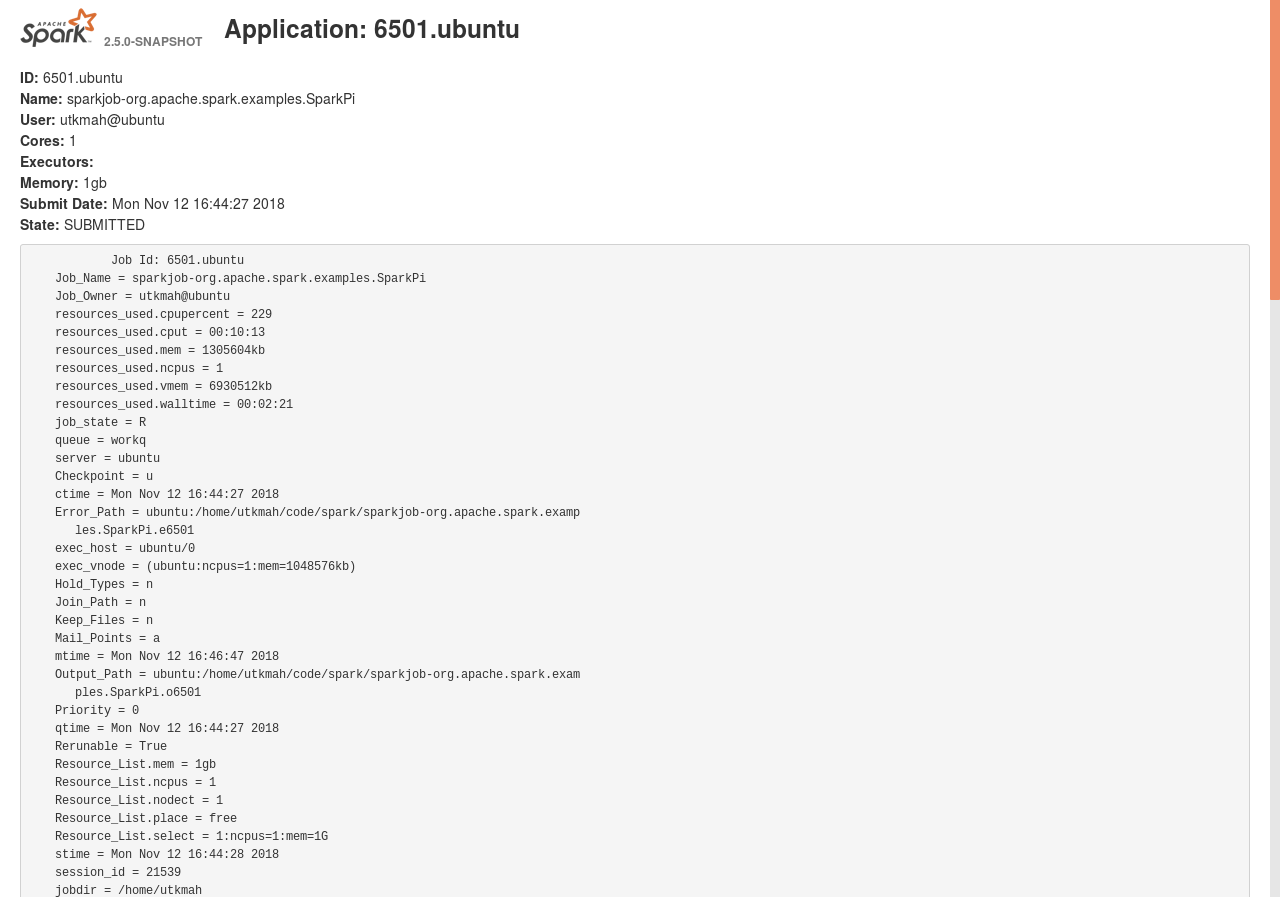
\includegraphics[width=0.75 \textwidth, natwidth=1280, natheight=897]
            {assets/images/App.png}
        }
    \caption{Spark Application page displaying PBS Job properties}
\end{figure}

\paragraph{}
In this prototype, the result for the \gls{spark} application has to be checked
using the PBS job logs as of now but that can be improved once the UI is in
place. The master UI can read the logs of the job and display them on the
application page in the webUI.


\chapter{Conclusions}
\section{client side change}
\section{issues}
\section{further scope of impovement}


\chapter{Appendices}
% vi:ft=tex

\section{Portable Batch System (PBS)}

\paragraph{} \glssymbol{pbs} is a workload management system that optimizes
\gls{job} scheduling based on computing resources like number of CPU cores,
memory, etc.


\subsection{Architecture}

\paragraph{} The \glssymbol{pbs} architecture consists of \textbf{Server},
\textbf{Scheduler}, \textbf{Comm} and \textbf{Machine Oriented Mini-server} or
MOM. In a typical \glssymbol{pbs} cluster, there can be only one Server, one
Comm, multiple Schedulers for different queues (based on priority, resources
etc.) and multiple MOMs (one for each node in the cluster).

\paragraph{} A PBS Server is responsible for taking a job from the client and
sending it to a scheduler. The scheduler then either puts the job in queue or
sends it to a MOM. The MOM is responsible to execute the job and return the
result back to the Server. The Comm is responsible for communication between
Server, Scheduler and MOMs.


\subsection{Job submission in PBS}

\paragraph{} The job submission in \glssymbol{pbs} is done via \texttt{qsub}
command. The parameters of a typical job submission include the number of CPU
cores, the amount of memory and the \gls{walltime} for the job.

\paragraph{} The jobs running at any given time can be checked via the command
\texttt{qstat}.



\newpage{}
\section{Apache Spark} \label{sec:appendix-spark}

\paragraph{} \gls{spark} is an engine for writing Big Data applications to
produce faster results on large quantities of data.


\subsection{Architecture}

\paragraph{} The \gls{spark} architecture consists of \textbf{Master} and
\textbf{Slave} daemons in the Spark Standalone Cluster Manager and
\textbf{\gls{driver}} and \textbf{\gls{executor}} which are two processes which
can run on the mentioned daemons.

\paragraph{Master and Slave Daemons} These are two daemons which are required to
be started before any application can be executed on a Spark Cluster. There can
be only one Master for each Spark Cluster and multiple Slaves (one for each node
in the cluster). These daemons are responsible for scheduling applications on
different nodes in the cluster. The Spark Applications are submitted to the
Master and run on Slaves.

\paragraph{\gls{driver} and \gls{executor}} These are two types of jobs which
can run on a \gls{spark} cluster. Every \gls{spark} application has a
\gls{driver} and multiple \glspl{executor}. A Driver is responsible for dividing
an application into several sub-tasks and scheduling these tasks on the
Executors. The Executors connect to the Driver, receive tasks from it, execute
the tasks and return the result back to it.


\subsection{Job submission in Spark}

\paragraph{} A \gls{spark} job is a program written in either Java, Scala,
Python or R. This program can be run interactively or in the background. The
application itself which is responsible for breaking the program into subtasks
and later assembling the result of the subtasks is called the \gls{driver}. When
the program is started in interactive mode (by specifying
\texttt{--deploy-mode client} or starting a shell), the driver is started on the
client node itself. When the application is submitted in non-interactive mode
(by specifying \texttt{--deploy-mode cluster}), the driver is started on a node
in the cluster itself.

\paragraph{} The \glspl{executor} are required to register to the \gls{driver}
to receive tasks and return results. This is achieved by creating an RPC
endpoint for each \gls{driver} to which the \glspl{executor} connect to. There
are two ways in which an \gls{executor} can associate with a \gls{driver}:

\paragraph{Coarse grained mode} In this mode, the \gls{executor} which is
started once is only stopped once the \gls{driver} ends or if it is explicitly
closed.

\paragraph{Fine grained mode} In this mode, the \gls{executor} is started and
stopped dynamically for each task.


\chapter{References}
% vi:ft=tex

\begin{description}[labelwidth=6cm]
    \item [PBS home page]
        \url{https://www.pbspro.org}

    \item [Spark home page]
        \url{https://spark.apache.org}

    \item [PBS contributor's portal]
        \url{https://pbspro.atlassian.net/wiki/spaces/PBSPro/overview}

    \item [Work repository]
        \url{https://github.com/UtkarshMe/Spark-PBSPro} 

    \item [Spark's bug-tracker ticket]
        \url{https://issues.apache.org/jira/browse/SPARK-25678} 

    \item [Pull request to Spark]
        \url{https://github.com/apache/spark/pull} 
\end{description}


\printglossaries
\addtocounter{chapter}{1}
\addcontentsline{toc}{chapter}{\protect\numberline{\thechapter}Glossary}

\end{document}
